


% Header, overrides base

    % Make sure that the sphinx doc style knows who it inherits from.
    \def\sphinxdocclass{article}

    % Declare the document class
    \documentclass[letterpaper,10pt,english]{/usr/local/lib/python2.7/dist-packages/sphinx/texinputs/sphinxhowto}

    % Imports
    \usepackage[utf8]{inputenc}
    \DeclareUnicodeCharacter{00A0}{\\nobreakspace}
    \usepackage[T1]{fontenc}
    \usepackage{babel}
    \usepackage{times}
    \usepackage{import}
    \usepackage[Bjarne]{/usr/local/lib/python2.7/dist-packages/sphinx/texinputs/fncychap}
    \usepackage{longtable}
    \usepackage{/usr/local/lib/python2.7/dist-packages/sphinx/texinputs/sphinx}
    \usepackage{multirow}

    \usepackage{amsmath}
    \usepackage{amssymb}
    \usepackage{ucs}
    \usepackage{enumerate}

    % Used to make the Input/Output rules follow around the contents.
    \usepackage{needspace}

    % Pygments requirements
    \usepackage{fancyvrb}
    \usepackage{color}
    % ansi colors additions
    \definecolor{darkgreen}{rgb}{.12,.54,.11}
    \definecolor{lightgray}{gray}{.95}
    \definecolor{brown}{rgb}{0.54,0.27,0.07}
    \definecolor{purple}{rgb}{0.5,0.0,0.5}
    \definecolor{darkgray}{gray}{0.25}
    \definecolor{lightred}{rgb}{1.0,0.39,0.28}
    \definecolor{lightgreen}{rgb}{0.48,0.99,0.0}
    \definecolor{lightblue}{rgb}{0.53,0.81,0.92}
    \definecolor{lightpurple}{rgb}{0.87,0.63,0.87}
    \definecolor{lightcyan}{rgb}{0.5,1.0,0.83}

    % Needed to box output/input
    \usepackage{tikz}
        \usetikzlibrary{calc,arrows,shadows}
    \usepackage[framemethod=tikz]{mdframed}

    \usepackage{alltt}

    % Used to load and display graphics
    \usepackage{graphicx}
    \graphicspath{ {figs/} }
    \usepackage[Export]{adjustbox} % To resize

    % used so that images for notebooks which have spaces in the name can still be included
    \usepackage{grffile}


    % For formatting output while also word wrapping.
    \usepackage{listings}
    \lstset{breaklines=true}
    \lstset{basicstyle=\small\ttfamily}
    \def\smaller{\fontsize{9.5pt}{9.5pt}\selectfont}

    %Pygments definitions
    
\makeatletter
\def\PY@reset{\let\PY@it=\relax \let\PY@bf=\relax%
    \let\PY@ul=\relax \let\PY@tc=\relax%
    \let\PY@bc=\relax \let\PY@ff=\relax}
\def\PY@tok#1{\csname PY@tok@#1\endcsname}
\def\PY@toks#1+{\ifx\relax#1\empty\else%
    \PY@tok{#1}\expandafter\PY@toks\fi}
\def\PY@do#1{\PY@bc{\PY@tc{\PY@ul{%
    \PY@it{\PY@bf{\PY@ff{#1}}}}}}}
\def\PY#1#2{\PY@reset\PY@toks#1+\relax+\PY@do{#2}}

\expandafter\def\csname PY@tok@gd\endcsname{\def\PY@tc##1{\textcolor[rgb]{0.63,0.00,0.00}{##1}}}
\expandafter\def\csname PY@tok@gu\endcsname{\let\PY@bf=\textbf\def\PY@tc##1{\textcolor[rgb]{0.50,0.00,0.50}{##1}}}
\expandafter\def\csname PY@tok@gt\endcsname{\def\PY@tc##1{\textcolor[rgb]{0.00,0.27,0.87}{##1}}}
\expandafter\def\csname PY@tok@gs\endcsname{\let\PY@bf=\textbf}
\expandafter\def\csname PY@tok@gr\endcsname{\def\PY@tc##1{\textcolor[rgb]{1.00,0.00,0.00}{##1}}}
\expandafter\def\csname PY@tok@cm\endcsname{\let\PY@it=\textit\def\PY@tc##1{\textcolor[rgb]{0.25,0.50,0.50}{##1}}}
\expandafter\def\csname PY@tok@vg\endcsname{\def\PY@tc##1{\textcolor[rgb]{0.10,0.09,0.49}{##1}}}
\expandafter\def\csname PY@tok@m\endcsname{\def\PY@tc##1{\textcolor[rgb]{0.40,0.40,0.40}{##1}}}
\expandafter\def\csname PY@tok@mh\endcsname{\def\PY@tc##1{\textcolor[rgb]{0.40,0.40,0.40}{##1}}}
\expandafter\def\csname PY@tok@go\endcsname{\def\PY@tc##1{\textcolor[rgb]{0.53,0.53,0.53}{##1}}}
\expandafter\def\csname PY@tok@ge\endcsname{\let\PY@it=\textit}
\expandafter\def\csname PY@tok@vc\endcsname{\def\PY@tc##1{\textcolor[rgb]{0.10,0.09,0.49}{##1}}}
\expandafter\def\csname PY@tok@il\endcsname{\def\PY@tc##1{\textcolor[rgb]{0.40,0.40,0.40}{##1}}}
\expandafter\def\csname PY@tok@cs\endcsname{\let\PY@it=\textit\def\PY@tc##1{\textcolor[rgb]{0.25,0.50,0.50}{##1}}}
\expandafter\def\csname PY@tok@cp\endcsname{\def\PY@tc##1{\textcolor[rgb]{0.74,0.48,0.00}{##1}}}
\expandafter\def\csname PY@tok@gi\endcsname{\def\PY@tc##1{\textcolor[rgb]{0.00,0.63,0.00}{##1}}}
\expandafter\def\csname PY@tok@gh\endcsname{\let\PY@bf=\textbf\def\PY@tc##1{\textcolor[rgb]{0.00,0.00,0.50}{##1}}}
\expandafter\def\csname PY@tok@ni\endcsname{\let\PY@bf=\textbf\def\PY@tc##1{\textcolor[rgb]{0.60,0.60,0.60}{##1}}}
\expandafter\def\csname PY@tok@nl\endcsname{\def\PY@tc##1{\textcolor[rgb]{0.63,0.63,0.00}{##1}}}
\expandafter\def\csname PY@tok@nn\endcsname{\let\PY@bf=\textbf\def\PY@tc##1{\textcolor[rgb]{0.00,0.00,1.00}{##1}}}
\expandafter\def\csname PY@tok@no\endcsname{\def\PY@tc##1{\textcolor[rgb]{0.53,0.00,0.00}{##1}}}
\expandafter\def\csname PY@tok@na\endcsname{\def\PY@tc##1{\textcolor[rgb]{0.49,0.56,0.16}{##1}}}
\expandafter\def\csname PY@tok@nb\endcsname{\def\PY@tc##1{\textcolor[rgb]{0.00,0.50,0.00}{##1}}}
\expandafter\def\csname PY@tok@nc\endcsname{\let\PY@bf=\textbf\def\PY@tc##1{\textcolor[rgb]{0.00,0.00,1.00}{##1}}}
\expandafter\def\csname PY@tok@nd\endcsname{\def\PY@tc##1{\textcolor[rgb]{0.67,0.13,1.00}{##1}}}
\expandafter\def\csname PY@tok@ne\endcsname{\let\PY@bf=\textbf\def\PY@tc##1{\textcolor[rgb]{0.82,0.25,0.23}{##1}}}
\expandafter\def\csname PY@tok@nf\endcsname{\def\PY@tc##1{\textcolor[rgb]{0.00,0.00,1.00}{##1}}}
\expandafter\def\csname PY@tok@si\endcsname{\let\PY@bf=\textbf\def\PY@tc##1{\textcolor[rgb]{0.73,0.40,0.53}{##1}}}
\expandafter\def\csname PY@tok@s2\endcsname{\def\PY@tc##1{\textcolor[rgb]{0.73,0.13,0.13}{##1}}}
\expandafter\def\csname PY@tok@vi\endcsname{\def\PY@tc##1{\textcolor[rgb]{0.10,0.09,0.49}{##1}}}
\expandafter\def\csname PY@tok@nt\endcsname{\let\PY@bf=\textbf\def\PY@tc##1{\textcolor[rgb]{0.00,0.50,0.00}{##1}}}
\expandafter\def\csname PY@tok@nv\endcsname{\def\PY@tc##1{\textcolor[rgb]{0.10,0.09,0.49}{##1}}}
\expandafter\def\csname PY@tok@s1\endcsname{\def\PY@tc##1{\textcolor[rgb]{0.73,0.13,0.13}{##1}}}
\expandafter\def\csname PY@tok@sh\endcsname{\def\PY@tc##1{\textcolor[rgb]{0.73,0.13,0.13}{##1}}}
\expandafter\def\csname PY@tok@sc\endcsname{\def\PY@tc##1{\textcolor[rgb]{0.73,0.13,0.13}{##1}}}
\expandafter\def\csname PY@tok@sx\endcsname{\def\PY@tc##1{\textcolor[rgb]{0.00,0.50,0.00}{##1}}}
\expandafter\def\csname PY@tok@bp\endcsname{\def\PY@tc##1{\textcolor[rgb]{0.00,0.50,0.00}{##1}}}
\expandafter\def\csname PY@tok@c1\endcsname{\let\PY@it=\textit\def\PY@tc##1{\textcolor[rgb]{0.25,0.50,0.50}{##1}}}
\expandafter\def\csname PY@tok@kc\endcsname{\let\PY@bf=\textbf\def\PY@tc##1{\textcolor[rgb]{0.00,0.50,0.00}{##1}}}
\expandafter\def\csname PY@tok@c\endcsname{\let\PY@it=\textit\def\PY@tc##1{\textcolor[rgb]{0.25,0.50,0.50}{##1}}}
\expandafter\def\csname PY@tok@mf\endcsname{\def\PY@tc##1{\textcolor[rgb]{0.40,0.40,0.40}{##1}}}
\expandafter\def\csname PY@tok@err\endcsname{\def\PY@bc##1{\setlength{\fboxsep}{0pt}\fcolorbox[rgb]{1.00,0.00,0.00}{1,1,1}{\strut ##1}}}
\expandafter\def\csname PY@tok@kd\endcsname{\let\PY@bf=\textbf\def\PY@tc##1{\textcolor[rgb]{0.00,0.50,0.00}{##1}}}
\expandafter\def\csname PY@tok@ss\endcsname{\def\PY@tc##1{\textcolor[rgb]{0.10,0.09,0.49}{##1}}}
\expandafter\def\csname PY@tok@sr\endcsname{\def\PY@tc##1{\textcolor[rgb]{0.73,0.40,0.53}{##1}}}
\expandafter\def\csname PY@tok@mo\endcsname{\def\PY@tc##1{\textcolor[rgb]{0.40,0.40,0.40}{##1}}}
\expandafter\def\csname PY@tok@kn\endcsname{\let\PY@bf=\textbf\def\PY@tc##1{\textcolor[rgb]{0.00,0.50,0.00}{##1}}}
\expandafter\def\csname PY@tok@mi\endcsname{\def\PY@tc##1{\textcolor[rgb]{0.40,0.40,0.40}{##1}}}
\expandafter\def\csname PY@tok@gp\endcsname{\let\PY@bf=\textbf\def\PY@tc##1{\textcolor[rgb]{0.00,0.00,0.50}{##1}}}
\expandafter\def\csname PY@tok@o\endcsname{\def\PY@tc##1{\textcolor[rgb]{0.40,0.40,0.40}{##1}}}
\expandafter\def\csname PY@tok@kr\endcsname{\let\PY@bf=\textbf\def\PY@tc##1{\textcolor[rgb]{0.00,0.50,0.00}{##1}}}
\expandafter\def\csname PY@tok@s\endcsname{\def\PY@tc##1{\textcolor[rgb]{0.73,0.13,0.13}{##1}}}
\expandafter\def\csname PY@tok@kp\endcsname{\def\PY@tc##1{\textcolor[rgb]{0.00,0.50,0.00}{##1}}}
\expandafter\def\csname PY@tok@w\endcsname{\def\PY@tc##1{\textcolor[rgb]{0.73,0.73,0.73}{##1}}}
\expandafter\def\csname PY@tok@kt\endcsname{\def\PY@tc##1{\textcolor[rgb]{0.69,0.00,0.25}{##1}}}
\expandafter\def\csname PY@tok@ow\endcsname{\let\PY@bf=\textbf\def\PY@tc##1{\textcolor[rgb]{0.67,0.13,1.00}{##1}}}
\expandafter\def\csname PY@tok@sb\endcsname{\def\PY@tc##1{\textcolor[rgb]{0.73,0.13,0.13}{##1}}}
\expandafter\def\csname PY@tok@k\endcsname{\let\PY@bf=\textbf\def\PY@tc##1{\textcolor[rgb]{0.00,0.50,0.00}{##1}}}
\expandafter\def\csname PY@tok@se\endcsname{\let\PY@bf=\textbf\def\PY@tc##1{\textcolor[rgb]{0.73,0.40,0.13}{##1}}}
\expandafter\def\csname PY@tok@sd\endcsname{\let\PY@it=\textit\def\PY@tc##1{\textcolor[rgb]{0.73,0.13,0.13}{##1}}}

\def\PYZbs{\char`\\}
\def\PYZus{\char`\_}
\def\PYZob{\char`\{}
\def\PYZcb{\char`\}}
\def\PYZca{\char`\^}
\def\PYZam{\char`\&}
\def\PYZlt{\char`\<}
\def\PYZgt{\char`\>}
\def\PYZsh{\char`\#}
\def\PYZpc{\char`\%}
\def\PYZdl{\char`\$}
\def\PYZhy{\char`\-}
\def\PYZsq{\char`\'}
\def\PYZdq{\char`\"}
\def\PYZti{\char`\~}
% for compatibility with earlier versions
\def\PYZat{@}
\def\PYZlb{[}
\def\PYZrb{]}
\makeatother


    %Set pygments styles if needed...
    
        \definecolor{nbframe-border}{rgb}{0.867,0.867,0.867}
        \definecolor{nbframe-bg}{rgb}{0.969,0.969,0.969}
        \definecolor{nbframe-in-prompt}{rgb}{0.0,0.0,0.502}
        \definecolor{nbframe-out-prompt}{rgb}{0.545,0.0,0.0}

        \newenvironment{ColorVerbatim}
        {\begin{mdframed}[%
            roundcorner=1.0pt, %
            backgroundcolor=nbframe-bg, %
            userdefinedwidth=1\linewidth, %
            leftmargin=0.1\linewidth, %
            innerleftmargin=0pt, %
            innerrightmargin=0pt, %
            linecolor=nbframe-border, %
            linewidth=1pt, %
            usetwoside=false, %
            everyline=true, %
            innerlinewidth=3pt, %
            innerlinecolor=nbframe-bg, %
            middlelinewidth=1pt, %
            middlelinecolor=nbframe-bg, %
            outerlinewidth=0.5pt, %
            outerlinecolor=nbframe-border, %
            needspace=0pt
        ]}
        {\end{mdframed}}
        
        \newenvironment{InvisibleVerbatim}
        {\begin{mdframed}[leftmargin=0.1\linewidth,innerleftmargin=3pt,innerrightmargin=3pt, userdefinedwidth=1\linewidth, linewidth=0pt, linecolor=white, usetwoside=false]}
        {\end{mdframed}}

        \renewenvironment{Verbatim}[1][\unskip]
        {\begin{alltt}\smaller}
        {\end{alltt}}
    

    % Help prevent overflowing lines due to urls and other hard-to-break 
    % entities.  This doesn't catch everything...
    \sloppy

    % Document level variables
    \title{Trabalho 1}
    \date{March 5, 2014}
    \release{}
    \author{Unknown Author}
    \renewcommand{\releasename}{}

    % TODO: Add option for the user to specify a logo for his/her export.
    \newcommand{\sphinxlogo}{}

    % Make the index page of the document.
    \makeindex

    % Import sphinx document type specifics.
     


% Body

    % Start of the document
    \begin{document}

        
            \maketitle
        

        


        
        \part{Função para carregamento de dados}
Função que carrega os dados dos arquivos, retornando dois arrays, um
contendo as n-1 primeiras colunas e outro com a n-ésima coluna.


    % Make sure that atleast 4 lines are below the HR
    \needspace{4\baselineskip}

    
        \vspace{6pt}
        \makebox[0.1\linewidth]{\smaller\hfill\tt\color{nbframe-in-prompt}In\hspace{4pt}{[}166{]}:\hspace{4pt}}\\*
        \vspace{-2.65\baselineskip}
        \begin{ColorVerbatim}
            \vspace{-0.7\baselineskip}
            \begin{Verbatim}[commandchars=\\\{\}]
\PY{n}{PATH\PYZus{}DADOS} \PY{o}{=} \PY{l+s}{\PYZdq{}}\PY{l+s}{Dados Exercicio 1}\PY{l+s}{\PYZdq{}}
\PY{n}{FILENAMES} \PY{o}{=} \PY{p}{[}\PY{l+s}{\PYZdq{}}\PY{l+s}{ex1data1.txt}\PY{l+s}{\PYZdq{}}\PY{p}{,} \PY{l+s}{\PYZdq{}}\PY{l+s}{ex1data2.txt}\PY{l+s}{\PYZdq{}}\PY{p}{,} \PY{l+s}{\PYZdq{}}\PY{l+s}{ex1data3.txt}\PY{l+s}{\PYZdq{}}\PY{p}{]}


\PY{k}{def} \PY{n+nf}{carregar}\PY{p}{(}\PY{n}{filename}\PY{p}{,} \PY{n}{delimiter}\PY{o}{=}\PY{l+s}{\PYZdq{}}\PY{l+s}{ }\PY{l+s}{\PYZdq{}}\PY{p}{)}\PY{p}{:}
    \PY{k+kn}{import} \PY{n+nn}{csv}
    \PY{k+kn}{import} \PY{n+nn}{os}
    
    \PY{n}{reader} \PY{o}{=} \PY{n}{csv}\PY{o}{.}\PY{n}{reader}\PY{p}{(}\PY{n+nb}{open}\PY{p}{(}\PY{n}{os}\PY{o}{.}\PY{n}{path}\PY{o}{.}\PY{n}{join}\PY{p}{(}\PY{n}{PATH\PYZus{}DADOS}\PY{p}{,} \PY{n}{filename}\PY{p}{)}\PY{p}{)}\PY{p}{,} \PY{n}{delimiter}\PY{o}{=}\PY{n}{delimiter}\PY{p}{)}
    
    \PY{n}{values\PYZus{}X} \PY{o}{=} \PY{p}{[}\PY{p}{]}
    \PY{n}{values\PYZus{}Y} \PY{o}{=} \PY{p}{[}\PY{p}{]}

    \PY{k}{for} \PY{n}{row} \PY{o+ow}{in} \PY{n}{reader}\PY{p}{:}
        \PY{n}{values\PYZus{}X}\PY{o}{.}\PY{n}{append}\PY{p}{(}\PY{p}{[}\PY{n+nb}{float}\PY{p}{(}\PY{n}{x}\PY{p}{)} \PY{k}{for} \PY{n}{x} \PY{o+ow}{in} \PY{n}{row}\PY{p}{[}\PY{p}{:}\PY{o}{\PYZhy{}}\PY{l+m+mi}{1}\PY{p}{]}\PY{p}{]}\PY{p}{)}
        \PY{n}{values\PYZus{}Y}\PY{o}{.}\PY{n}{append}\PY{p}{(}\PY{n+nb}{float}\PY{p}{(}\PY{n}{row}\PY{p}{[}\PY{o}{\PYZhy{}}\PY{l+m+mi}{1}\PY{p}{]}\PY{p}{)}\PY{p}{)}
    
    \PY{k+kn}{import} \PY{n+nn}{numpy} \PY{k+kn}{as} \PY{n+nn}{np}

    \PY{k}{return} \PY{n}{np}\PY{o}{.}\PY{n}{array}\PY{p}{(}\PY{n}{values\PYZus{}X}\PY{p}{)}\PY{p}{,} \PY{n}{np}\PY{o}{.}\PY{n}{array}\PY{p}{(}\PY{n}{values\PYZus{}Y}\PY{p}{)}
\end{Verbatim}

            
                \vspace{-0.2\baselineskip}
            
        \end{ColorVerbatim}
    
\part{Função para plotar o gráfico com duas dimensões}

    % Make sure that atleast 4 lines are below the HR
    \needspace{4\baselineskip}

    
        \vspace{6pt}
        \makebox[0.1\linewidth]{\smaller\hfill\tt\color{nbframe-in-prompt}In\hspace{4pt}{[}194{]}:\hspace{4pt}}\\*
        \vspace{-2.65\baselineskip}
        \begin{ColorVerbatim}
            \vspace{-0.7\baselineskip}
            \begin{Verbatim}[commandchars=\\\{\}]
\PY{k}{def} \PY{n+nf}{plot2d}\PY{p}{(}\PY{n}{X}\PY{p}{,} \PY{n}{Y}\PY{p}{,} \PY{n}{color}\PY{o}{=}\PY{n+nb+bp}{None}\PY{p}{)}\PY{p}{:}
    \PY{k+kn}{from} \PY{n+nn}{matplotlib} \PY{k+kn}{import} \PY{n}{pyplot} \PY{k}{as} \PY{n}{pl}
        
    \PY{n}{line} \PY{o}{=} \PY{n}{pl}\PY{o}{.}\PY{n}{plot}\PY{p}{(}\PY{n}{X}\PY{p}{,} \PY{n}{Y}\PY{p}{)}
    \PY{k}{if} \PY{o+ow}{not} \PY{n}{color} \PY{o+ow}{is} \PY{n+nb+bp}{None}\PY{p}{:}
        \PY{n}{pyplot}\PY{o}{.}\PY{n}{setp}\PY{p}{(}\PY{n}{line}\PY{p}{,} \PY{n}{color}\PY{o}{=}\PY{n}{color}\PY{p}{)}

\PY{k}{def} \PY{n+nf}{scatter2d}\PY{p}{(}\PY{n}{X}\PY{p}{,} \PY{n}{Y}\PY{p}{)}\PY{p}{:}
    \PY{k+kn}{from} \PY{n+nn}{matplotlib} \PY{k+kn}{import} \PY{n}{pyplot} \PY{k}{as} \PY{n}{pl}
    
    \PY{n}{pl}\PY{o}{.}\PY{n}{scatter}\PY{p}{(}\PY{n}{X}\PY{p}{,} \PY{n}{Y}\PY{p}{)}
\end{Verbatim}

            
                \vspace{-0.2\baselineskip}
            
        \end{ColorVerbatim}
    
\part{Questão 1}\subsubsection{Figura com os dados}

    % Make sure that atleast 4 lines are below the HR
    \needspace{4\baselineskip}

    
        \vspace{6pt}
        \makebox[0.1\linewidth]{\smaller\hfill\tt\color{nbframe-in-prompt}In\hspace{4pt}{[}206{]}:\hspace{4pt}}\\*
        \vspace{-2.65\baselineskip}
        \begin{ColorVerbatim}
            \vspace{-0.7\baselineskip}
            \begin{Verbatim}[commandchars=\\\{\}]
\PY{n}{X}\PY{p}{,} \PY{n}{Y} \PY{o}{=} \PY{n}{carregar}\PY{p}{(}\PY{n}{FILENAMES}\PY{p}{[}\PY{l+m+mi}{0}\PY{p}{]}\PY{p}{)}
\PY{n}{scatter2d}\PY{p}{(}\PY{n}{X}\PY{p}{,} \PY{n}{Y}\PY{p}{)}
\end{Verbatim}

            
                \vspace{-0.2\baselineskip}
            
        \end{ColorVerbatim}
    

    

        % If the first block is an image, minipage the image.  Else
        % request a certain amount of space for the input text.
        \needspace{4\baselineskip}
        
        

            % Add document contents.
            
                \begin{InvisibleVerbatim}
                \vspace{-0.5\baselineskip}
\begin{alltt}[17.592, 9.1302, 13.662, 11.854, 6.8233, 11.886, 4.3483, 12.0, 6.5987,
3.8166, 3.2522, 15.505, 3.1551, 7.2258, 0.71618, 3.5129, 5.3048,
0.56077, 3.6518, 5.3893, 3.1386, 21.767, 4.263, 5.1875, 3.0825,
22.638, 13.501, 7.0467, 14.692, 24.147, -1.22, 5.9966, 12.134, 1.8495,
6.5426, 4.5623, 4.1164, 3.3928, 10.117, 5.4974, 0.55657, 3.9115,
5.3854, 2.4406, 6.7318, 1.0463, 5.1337, 1.844, 8.0043, 1.0179, 6.7504,
1.8396, 4.2885, 4.9981, 1.4233, -1.4211, 2.4756, 4.6042, 3.9624,
5.4141, 5.1694, -0.74279, 17.929, 12.054, 17.054, 4.8852, 5.7442,
7.7754, 1.0173, 20.992, 6.6799, 4.0259, 1.2784, 3.3411, -2.6807,
0.29678, 3.8845, 5.7014, 6.7526, 2.0576, 0.47953, 0.20421, 0.67861,
7.5435, 5.3436, 4.2415, 6.7981, 0.92695, 0.152, 2.8214, 1.8451,
4.2959, 7.2029, 1.9869, 0.14454, 9.0551, 0.61705]
\end{alltt}

            \end{InvisibleVerbatim}
            
                \begin{InvisibleVerbatim}
                \vspace{-0.5\baselineskip}
    \begin{center}
    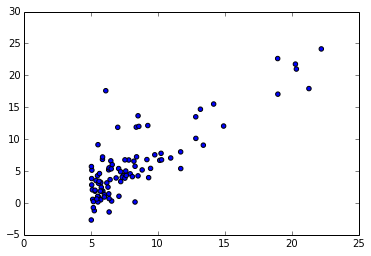
\includegraphics[max size={\textwidth}{\textheight}]{Trabalho 1_files/Trabalho 1_7_1.png}
    \par
    \end{center}
    
            \end{InvisibleVerbatim}
            
        
    
\subsubsection{Comentários: Um modelo de regressão linear parece ser adequado para os
dados em questão? Comente.}
Essa questão só pode ser respondida a partir da definição de
"adequado". Ela envolve aspectos como a precisão que se deseja
alcançar com o modelo e quão próximo dos dados de treinamento espera-
se que os dados a serem predizidos sejam.
Pelo gráfico, os dados não parecem possuir uma boa aproximação por uma
reta, por possuir, para valores próximos de x, variações não
monotônicas de y.
\subsubsection{\begin{itemize}
\itemsep1pt\parskip0pt\parsep0pt
\item
  Implemente o algoritmo do gradiente descendente estocástico para
  encontrar os coeficientes da regressão.
\end{itemize}}

    % Make sure that atleast 4 lines are below the HR
    \needspace{4\baselineskip}

    
        \vspace{6pt}
        \makebox[0.1\linewidth]{\smaller\hfill\tt\color{nbframe-in-prompt}In\hspace{4pt}{[}207{]}:\hspace{4pt}}\\*
        \vspace{-2.65\baselineskip}
        \begin{ColorVerbatim}
            \vspace{-0.7\baselineskip}
            \begin{Verbatim}[commandchars=\\\{\}]
\PY{c}{\PYZsh{} retorna o EQM, a média dos erros e a média dos erros pelos x\PYZsq{}s}
\PY{k}{def} \PY{n+nf}{eqm}\PY{p}{(}\PY{n}{x}\PY{p}{,} \PY{n}{gerado}\PY{p}{,} \PY{n}{esperado}\PY{p}{)}\PY{p}{:}
    \PY{n}{resultado} \PY{o}{=} \PY{l+m+mf}{0.}
    
    \PY{k}{for} \PY{n}{g}\PY{p}{,} \PY{n}{e} \PY{o+ow}{in} \PY{n+nb}{zip}\PY{p}{(}\PY{n}{gerado}\PY{p}{,} \PY{n}{esperado}\PY{p}{)}\PY{p}{:}
        \PY{n}{erro} \PY{o}{=} \PY{n}{g} \PY{o}{\PYZhy{}} \PY{n}{e}
        \PY{n}{erro\PYZus{}quadrado} \PY{o}{=} \PY{n}{erro}\PY{o}{*}\PY{o}{*}\PY{l+m+mi}{2}
        
        \PY{n}{resultado} \PY{o}{+}\PY{o}{=} \PY{n}{erro\PYZus{}quadrado}
        
    \PY{n}{resultado} \PY{o}{/}\PY{o}{=} \PY{n+nb}{len}\PY{p}{(}\PY{n}{gerado}\PY{p}{)}
    
    \PY{k}{return} \PY{n}{resultado}

\PY{k}{def} \PY{n+nf}{eq\PYZus{}1grau}\PY{p}{(}\PY{n}{w0}\PY{p}{,} \PY{n}{w1}\PY{p}{,} \PY{n}{x}\PY{p}{)}\PY{p}{:}
    
    \PY{k}{return} \PY{n}{w0} \PY{o}{+} \PY{n}{w1}\PY{o}{*}\PY{n}{x}
    

\PY{k}{def} \PY{n+nf}{grad\PYZus{}desc\PYZus{}estoq\PYZus{}univ}\PY{p}{(}\PY{n}{X}\PY{p}{,} \PY{n}{Y}\PY{p}{,} \PY{n}{alfa}\PY{o}{=}\PY{l+m+mf}{0.1}\PY{p}{,} \PY{n}{epocas}\PY{o}{=}\PY{l+m+mi}{100}\PY{p}{,} \PY{n}{w0} \PY{o}{=} \PY{n+nb+bp}{None}\PY{p}{,} \PY{n}{w1} \PY{o}{=} \PY{n+nb+bp}{None}\PY{p}{,} \PY{n}{plot}\PY{o}{=}\PY{n+nb+bp}{False}\PY{p}{)}\PY{p}{:}
    \PY{c}{\PYZsh{} valores randomicos para w0 e w1}
    \PY{k}{if} \PY{n}{w0} \PY{o+ow}{is} \PY{n+nb+bp}{None}\PY{p}{:}
        \PY{n}{w0} \PY{o}{=} \PY{n}{random}\PY{o}{.}\PY{n}{uniform}\PY{p}{(}\PY{l+m+mi}{1}\PY{p}{,} \PY{l+m+mi}{10}\PY{p}{)}
    \PY{k}{if} \PY{n}{w1} \PY{o+ow}{is} \PY{n+nb+bp}{None}\PY{p}{:}
        \PY{n}{w1} \PY{o}{=} \PY{n}{random}\PY{o}{.}\PY{n}{uniform}\PY{p}{(}\PY{l+m+mi}{1}\PY{p}{,} \PY{l+m+mi}{10}\PY{p}{)}
    
    \PY{n}{eqms} \PY{o}{=} \PY{p}{[}\PY{p}{]}
    
    \PY{c}{\PYZsh{} percorre os valores de x e y}
    \PY{k+kn}{from} \PY{n+nn}{itertools} \PY{k+kn}{import} \PY{n}{cycle}
    \PY{n}{xs} \PY{o}{=} \PY{n}{cycle}\PY{p}{(}\PY{n}{X}\PY{p}{)}
    \PY{n}{ys} \PY{o}{=} \PY{n}{cycle}\PY{p}{(}\PY{n}{Y}\PY{p}{)}
    
    \PY{k}{for} \PY{n}{epoca}\PY{p}{,} \PY{n}{x}\PY{p}{,} \PY{n}{y} \PY{o+ow}{in} \PY{n+nb}{zip}\PY{p}{(}\PY{n+nb}{xrange}\PY{p}{(}\PY{n}{epocas}\PY{p}{)}\PY{p}{,} \PY{n}{xs}\PY{p}{,} \PY{n}{ys}\PY{p}{)}\PY{p}{:}
        \PY{c}{\PYZsh{} calcula as predições para os dados de treinamento}
        \PY{n}{predicao} \PY{o}{=} \PY{p}{[}\PY{n}{eq\PYZus{}1grau}\PY{p}{(}\PY{n}{w0}\PY{p}{,} \PY{n}{w1}\PY{p}{,} \PY{n}{elem}\PY{p}{[}\PY{l+m+mi}{0}\PY{p}{]}\PY{p}{)} \PY{k}{for} \PY{n}{elem} \PY{o+ow}{in} \PY{n}{X}\PY{p}{]}
        
        \PY{c}{\PYZsh{} calcula o eqm}
        \PY{n}{eqm\PYZus{}calculado} \PY{o}{=} \PY{n}{eqm}\PY{p}{(}\PY{n}{X}\PY{p}{,} \PY{n}{predicao}\PY{p}{,} \PY{n}{Y}\PY{p}{)}
        \PY{n}{eqms}\PY{o}{.}\PY{n}{append}\PY{p}{(}\PY{n}{eqm\PYZus{}calculado}\PY{p}{)}
        
        \PY{c}{\PYZsh{} erro da iteração}
        \PY{n}{erro} \PY{o}{=} \PY{n}{y} \PY{o}{\PYZhy{}} \PY{n}{eq\PYZus{}1grau}\PY{p}{(}\PY{n}{w0}\PY{p}{,} \PY{n}{w1}\PY{p}{,} \PY{n}{x}\PY{p}{[}\PY{l+m+mi}{0}\PY{p}{]}\PY{p}{)}
        \PY{c}{\PYZsh{} atualiza os pesos}
        \PY{n}{w0} \PY{o}{+}\PY{o}{=} \PY{n}{alfa}\PY{o}{*}\PY{n}{erro}
        \PY{n}{w1} \PY{o}{+}\PY{o}{=} \PY{n}{alfa}\PY{o}{*}\PY{n}{erro}\PY{o}{*}\PY{n}{x}\PY{p}{[}\PY{l+m+mi}{0}\PY{p}{]}
        
    \PY{k}{if} \PY{n}{plot}\PY{p}{:}
        \PY{n}{scatter2d}\PY{p}{(}\PY{n}{X}\PY{p}{,} \PY{n}{Y}\PY{p}{)}
        \PY{n}{plot2d}\PY{p}{(}\PY{n}{X}\PY{p}{,} \PY{p}{[}\PY{n}{eq\PYZus{}1grau}\PY{p}{(}\PY{n}{w0}\PY{p}{,} \PY{n}{w1}\PY{p}{,} \PY{n}{x}\PY{p}{[}\PY{l+m+mi}{0}\PY{p}{]}\PY{p}{)} \PY{k}{for} \PY{n}{x} \PY{o+ow}{in} \PY{n}{X}\PY{p}{]}\PY{p}{,} \PY{n}{color}\PY{o}{=}\PY{l+s}{\PYZdq{}}\PY{l+s}{r}\PY{l+s}{\PYZdq{}}\PY{p}{)}
        
    \PY{k}{return} \PY{n}{w0}\PY{p}{,} \PY{n}{w1}\PY{p}{,} \PY{n}{eqms}
    
\end{Verbatim}

            
                \vspace{-0.2\baselineskip}
            
        \end{ColorVerbatim}
    
\subsubsection{Cálculo dos pesos e dos EQMs}

    % Make sure that atleast 4 lines are below the HR
    \needspace{4\baselineskip}

    
        \vspace{6pt}
        \makebox[0.1\linewidth]{\smaller\hfill\tt\color{nbframe-in-prompt}In\hspace{4pt}{[}208{]}:\hspace{4pt}}\\*
        \vspace{-2.65\baselineskip}
        \begin{ColorVerbatim}
            \vspace{-0.7\baselineskip}
            \begin{Verbatim}[commandchars=\\\{\}]
\PY{n}{w0}\PY{p}{,} \PY{n}{w1}\PY{p}{,} \PY{n}{eqms} \PY{o}{=} \PY{n}{grad\PYZus{}desc\PYZus{}estoq\PYZus{}univ}\PY{p}{(}\PY{n}{X}\PY{p}{,} \PY{n}{Y}\PY{p}{,} \PY{n}{alfa}\PY{o}{=}\PY{l+m+mf}{0.001}\PY{p}{,} \PY{n}{epocas}\PY{o}{=}\PY{l+m+mi}{1000}\PY{p}{)}
\end{Verbatim}

            
                \vspace{-0.2\baselineskip}
            
        \end{ColorVerbatim}
    
\subsubsection{Plot do gráfico de EQM por época}

    % Make sure that atleast 4 lines are below the HR
    \needspace{4\baselineskip}

    
        \vspace{6pt}
        \makebox[0.1\linewidth]{\smaller\hfill\tt\color{nbframe-in-prompt}In\hspace{4pt}{[}209{]}:\hspace{4pt}}\\*
        \vspace{-2.65\baselineskip}
        \begin{ColorVerbatim}
            \vspace{-0.7\baselineskip}
            \begin{Verbatim}[commandchars=\\\{\}]
\PY{n}{plot2d}\PY{p}{(}\PY{n+nb}{xrange}\PY{p}{(}\PY{n+nb}{len}\PY{p}{(}\PY{n}{eqms}\PY{p}{)}\PY{p}{)}\PY{p}{,} \PY{n}{eqms}\PY{p}{)}
\end{Verbatim}

            
                \vspace{-0.2\baselineskip}
            
        \end{ColorVerbatim}
    

    

        % If the first block is an image, minipage the image.  Else
        % request a certain amount of space for the input text.
        \needspace{4\baselineskip}
        
        

            % Add document contents.
            
                \begin{InvisibleVerbatim}
                \vspace{-0.5\baselineskip}
    \begin{center}
    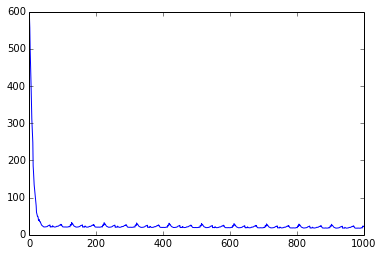
\includegraphics[max size={\textwidth}{\textheight}]{Trabalho 1_files/Trabalho 1_15_0.png}
    \par
    \end{center}
    
            \end{InvisibleVerbatim}
            
        
    
\subsubsection{Valor final dos coeficientes}

    % Make sure that atleast 4 lines are below the HR
    \needspace{4\baselineskip}

    
        \vspace{6pt}
        \makebox[0.1\linewidth]{\smaller\hfill\tt\color{nbframe-in-prompt}In\hspace{4pt}{[}210{]}:\hspace{4pt}}\\*
        \vspace{-2.65\baselineskip}
        \begin{ColorVerbatim}
            \vspace{-0.7\baselineskip}
            \begin{Verbatim}[commandchars=\\\{\}]
\PY{k}{print} \PY{l+s}{\PYZdq{}}\PY{l+s}{w0 =}\PY{l+s}{\PYZdq{}}\PY{p}{,} \PY{n}{w0}\PY{p}{,} \PY{l+s}{\PYZdq{}}\PY{l+s}{w1 =}\PY{l+s}{\PYZdq{}}\PY{p}{,} \PY{n}{w1}
\end{Verbatim}

            
                \vspace{-0.2\baselineskip}
            
        \end{ColorVerbatim}
    

    

        % If the first block is an image, minipage the image.  Else
        % request a certain amount of space for the input text.
        \needspace{4\baselineskip}
        
        

            % Add document contents.
            
                \begin{InvisibleVerbatim}
                \vspace{-0.5\baselineskip}
\begin{alltt}w0 = 3.05900253324 w1 = 0.845344711405
\end{alltt}

            \end{InvisibleVerbatim}
            
        
    
\subsubsection{Comentários: Através do gráfico ``épocas x EQM'' é possível verificar
que o algoritmo está ``aprendendo'' ? Comente.}
Considerando que uma diminuição dos erros do modelo em predições sobre
dados do training-set representam aprendizado, pode-se sim afirmar que
o  algoritmo está "aprendendo".
Podemos pensar cada época de treinamento como um incremento no
aprendizado.
\subsubsection{Exemplo de utilização da função, para um conjunto de dados
simples(função 2*x)}

    % Make sure that atleast 4 lines are below the HR
    \needspace{4\baselineskip}

    
        \vspace{6pt}
        \makebox[0.1\linewidth]{\smaller\hfill\tt\color{nbframe-in-prompt}In\hspace{4pt}{[}211{]}:\hspace{4pt}}\\*
        \vspace{-2.65\baselineskip}
        \begin{ColorVerbatim}
            \vspace{-0.7\baselineskip}
            \begin{Verbatim}[commandchars=\\\{\}]
\PY{n}{w0}\PY{p}{,} \PY{n}{w1}\PY{p}{,} \PY{n}{eqms} \PY{o}{=} \PY{n}{grad\PYZus{}desc\PYZus{}estoq\PYZus{}univ}\PY{p}{(}\PY{p}{[}\PY{p}{[}\PY{n}{x}\PY{p}{]} \PY{k}{for} \PY{n}{x} \PY{o+ow}{in} \PY{n+nb}{xrange}\PY{p}{(}\PY{l+m+mi}{40}\PY{p}{)}\PY{p}{]}\PY{p}{,} \PY{p}{[}\PY{l+m+mi}{2}\PY{o}{*}\PY{n}{x} \PY{k}{for} \PY{n}{x} \PY{o+ow}{in} \PY{n+nb}{xrange}\PY{p}{(}\PY{l+m+mi}{40}\PY{p}{)}\PY{p}{]}\PY{p}{,} \PY{n}{alfa}\PY{o}{=}\PY{l+m+mf}{0.001}\PY{p}{,} \PY{n}{epocas}\PY{o}{=}\PY{l+m+mi}{1000}\PY{p}{,} \PY{n}{plot}\PY{o}{=}\PY{n+nb+bp}{True}\PY{p}{)}
\end{Verbatim}

            
                \vspace{-0.2\baselineskip}
            
        \end{ColorVerbatim}
    

    

        % If the first block is an image, minipage the image.  Else
        % request a certain amount of space for the input text.
        \needspace{4\baselineskip}
        
        

            % Add document contents.
            
                \begin{InvisibleVerbatim}
                \vspace{-0.5\baselineskip}
    \begin{center}
    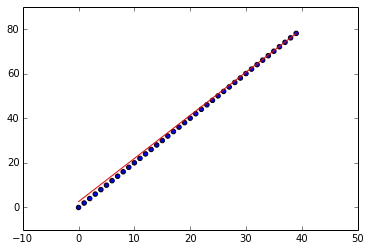
\includegraphics[max size={\textwidth}{\textheight}]{Trabalho 1_files/Trabalho 1_21_0.png}
    \par
    \end{center}
    
            \end{InvisibleVerbatim}
            
        
    


    % Make sure that atleast 4 lines are below the HR
    \needspace{4\baselineskip}

    
        \vspace{6pt}
        \makebox[0.1\linewidth]{\smaller\hfill\tt\color{nbframe-in-prompt}In\hspace{4pt}{[}212{]}:\hspace{4pt}}\\*
        \vspace{-2.65\baselineskip}
        \begin{ColorVerbatim}
            \vspace{-0.7\baselineskip}
            \begin{Verbatim}[commandchars=\\\{\}]
\PY{n}{plot2d}\PY{p}{(}\PY{n+nb}{xrange}\PY{p}{(}\PY{n+nb}{len}\PY{p}{(}\PY{n}{eqms}\PY{p}{)}\PY{p}{)}\PY{p}{,} \PY{n}{eqms}\PY{p}{)}
\end{Verbatim}

            
                \vspace{-0.2\baselineskip}
            
        \end{ColorVerbatim}
    

    

        % If the first block is an image, minipage the image.  Else
        % request a certain amount of space for the input text.
        \needspace{4\baselineskip}
        
        

            % Add document contents.
            
                \begin{InvisibleVerbatim}
                \vspace{-0.5\baselineskip}
    \begin{center}
    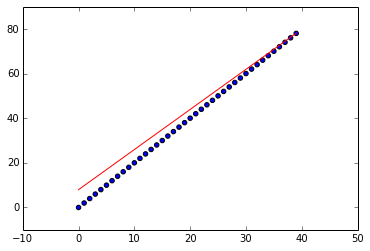
\includegraphics[max size={\textwidth}{\textheight}]{Trabalho 1_files/Trabalho 1_22_0.png}
    \par
    \end{center}
    
            \end{InvisibleVerbatim}
            
        
    
\subsubsection{Utilizando o modelo do scikit-learn}

    % Make sure that atleast 4 lines are below the HR
    \needspace{4\baselineskip}

    
        \vspace{6pt}
        \makebox[0.1\linewidth]{\smaller\hfill\tt\color{nbframe-in-prompt}In\hspace{4pt}{[}213{]}:\hspace{4pt}}\\*
        \vspace{-2.65\baselineskip}
        \begin{ColorVerbatim}
            \vspace{-0.7\baselineskip}
            \begin{Verbatim}[commandchars=\\\{\}]
\PY{k+kn}{from} \PY{n+nn}{sklearn} \PY{k+kn}{import} \PY{n}{linear\PYZus{}model}
\PY{n}{clf} \PY{o}{=} \PY{n}{linear\PYZus{}model}\PY{o}{.}\PY{n}{LinearRegression}\PY{p}{(}\PY{p}{)}
\PY{n}{clf}\PY{o}{.}\PY{n}{fit}\PY{p}{(}\PY{p}{[}\PY{p}{[}\PY{n}{x}\PY{p}{]} \PY{k}{for} \PY{n}{x} \PY{o+ow}{in} \PY{n+nb}{xrange}\PY{p}{(}\PY{l+m+mi}{20}\PY{p}{)}\PY{p}{]}\PY{p}{,} \PY{p}{[}\PY{n}{x}\PY{o}{*}\PY{l+m+mi}{2} \PY{o}{+} \PY{l+m+mi}{4} \PY{k}{for} \PY{n}{x} \PY{o+ow}{in} \PY{n+nb}{xrange}\PY{p}{(}\PY{l+m+mi}{20}\PY{p}{)}\PY{p}{]}\PY{p}{)}

\PY{k}{print} \PY{n}{clf}\PY{o}{.}\PY{n}{coef\PYZus{}}
\end{Verbatim}

            
                \vspace{-0.2\baselineskip}
            
        \end{ColorVerbatim}
    

    

        % If the first block is an image, minipage the image.  Else
        % request a certain amount of space for the input text.
        \needspace{4\baselineskip}
        
        

            % Add document contents.
            
                \begin{InvisibleVerbatim}
                \vspace{-0.5\baselineskip}
\begin{alltt}[ 2.]
\end{alltt}

            \end{InvisibleVerbatim}
            
        
    

        

        \renewcommand{\indexname}{Index}
        \printindex

    % End of document
    \end{document}


